%%%%%%%%%%%%%%%%%%%%%%%%%%%%%%%%%%%%%%%%%
% baposter Portrait Poster
% LaTeX Template
% Version 1.0 (15/5/13)
%
% Created by:
% Brian Amberg (baposter@brian-amberg.de)
%
% This template has been downloaded from:
% http://www.LaTeXTemplates.com
%
% License:
% CC BY-NC-SA 3.0 (http://creativecommons.org/licenses/by-nc-sa/3.0/)
%
%%%%%%%%%%%%%%%%%%%%%%%%%%%%%%%%%%%%%%%%%

%----------------------------------------------------------------------------------------
%	PACKAGES AND OTHER DOCUMENT CONFIGURATIONS
%----------------------------------------------------------------------------------------

\documentclass[paperwidth=137.2cm,paperheight=91.4cm]{baposter}

\usepackage[font=footnotesize,labelfont=bf]{caption} % Required for specifying captions to tables and figures
\usepackage{booktabs} % Horizontal rules in tables
\usepackage{relsize} % Used for making text smaller in some places
\usepackage[utf8x]{inputenc}
\usepackage[superscript,biblabel]{cite}
\usepackage{tikz}
\usepackage{dsfont}
\usepackage{cmbright}
\usepackage[T1]{fontenc}

\graphicspath{{figures/}} % Directory in which figures are stored

\definecolor{bordercol}{RGB}{40,40,40} % Border color of content boxes
\definecolor{headercol1}{RGB}{255,255,255} % Background color for the header in the content boxes (left side)
\definecolor{headercol2}{RGB}{255,255,255} % Background color for the header in the content boxes (right side)
\definecolor{headerfontcol}{HTML}{E6002E} % Text color for the header text in the content boxes
\definecolor{boxcolor}{RGB}{255,255,255} % Background color for the content in the content boxes

\definecolor{ubRed}{HTML}{E6002E}
\definecolor{maroon}{RGB}{176, 48, 96}
\definecolor{orange2}{RGB}{238, 118, 0}
\newcommand{\alert}[1]{\textbf{#1}}
\newcommand{\colindic}[1]{\textcolor{maroon}{#1}}
\newcommand{\colsurvey}[1]{\textcolor{orange2}{#1}}

\begin{document}

\background{ % Set the background to an image (background.pdf)
\begin{tikzpicture}[remember picture,overlay]
\draw (current page.north west)+(-2em,2em) node[anchor=north west]
{
\includegraphics[height=1.1\textheight]{background.pdf}};
\end{tikzpicture}
}

\begin{poster}{
grid=false,
borderColor=bordercol, % Border color of content boxes
headerColorOne=headercol1, % Background color for the header in the content boxes (left side)
headerColorTwo=headercol2, % Background color for the header in the content boxes (right side)
headerFontColor=headerfontcol, % Text color for the header text in the content boxes
boxColorOne=boxcolor, % Background color for the content in the content boxes
headershape=roundedright, % Specify the rounded corner in the content box headers
headerfont=\Large\sf\bf, % Font modifiers for the text in the content box headers
textborder=rectangle,
background=user,
headerborder=open, % Change to closed for a line under the content box headers
boxshade=plain,
columns=5
}
{}
%
%----------------------------------------------------------------------------------------
%	TITLE AND AUTHOR NAME
%----------------------------------------------------------------------------------------
%
{\sf\bf \Huge{ Drivers of NNRTI resistance in Southern Africa }\vspace{.1em}} % Poster title
{ \underline{Julien Riou}\textsuperscript{1}, Carole Dupont\textsuperscript{1}, Silvia Bertagnolio\textsuperscript{2}, Ravindra K.~Gupta\textsuperscript{3}, Leigh F.~Johnson\textsuperscript{4}, Roger D.~Kouyos\textsuperscript{5}, Matthias Egger\textsuperscript{1,4}, Christian L.~Althaus\textsuperscript{1}\\ \vspace{.2em} % Author names
{\smaller \textit{ \textsuperscript{1}Institute of Social and Preventive Medicine, University of Bern, Switzerland; 
	\textsuperscript{2}HIV/Hepatitis/STI Department, WHO; \textsuperscript{3}Department of Infection, University College London, UK and Africa Health Research Institute, South Africa; \textsuperscript{4}CIDER, University of Cape Town, South Africa;  \textsuperscript{5}University Hospital Zurich and Institute of Medical Virology, University of Zurich, Switzerland. }}} % Author email addresses
{1506\hspace{.5cm} 
\includegraphics[height=6em]{figures/ideasa2.png} } % University/lab logo

%----------------------------------------------------------------------------------------
%	INTRODUCTION
%----------------------------------------------------------------------------------------

\headerbox{Background}{name=introduction,column=0,row=0}{
\begin{flushleft}
	The rise of HIV-1 drug resistance to \alert{non-nucleoside reverse-transcriptase inhibitors} (NNRTI) threatens the success of antiretroviral therapy (ART) in southern Africa:
	\vspace{-.5em}
	\begin{itemize}
		\item low genetic barrier to resistance \vspace{-.5em}
		\item poor adherence, bad prescription practices, supply chains... 
	\end{itemize}
	HIV drug resistance is assessed by monitoring \alert{pretreatment drug resistance} (PDR): the proportion of resistance mutations among ART-naïve individuals.
\end{flushleft}
	\vspace{.1em}
}

%----------------------------------------------------------------------------------------
%	MATERIALS AND METHODS
%----------------------------------------------------------------------------------------

\headerbox{Increasing PDR in the region}{name=growing,column=0,below=introduction}{
\begin{flushleft}
	Systematic review of PDR surveys in adults \alert{by region} until 2016:
	\begin{center}
		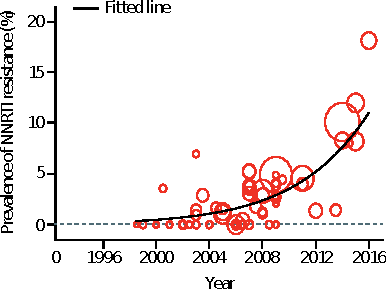
\includegraphics[width=.7\linewidth]{figures/Gupta2018.pdf}
		\captionof{figure}{NNRTI PDR from surveys conducted in 9 countries of \alert{southern Africa } (Gupta et al., 2018).}
	\end{center}
\end{flushleft}
}

%----------------------------------------------------------------------------------------
%	OBJECTIVES
%----------------------------------------------------------------------------------------

\headerbox{Objectives}{name=objectives,column=0,below=growing}{
	\begin{flushleft}
	
	1. \alert{Estimate} the emergence of NNRTI resistance across countries accounting for the local dynamics of HIV-1 transmission, treatment and mortality. \vspace{.65em}
	
	2. Conduct between-country \alert{comparisons}.\vspace{.65em}
	
	3. Identify \alert{potential drivers} at the country level.

	
	\begin{center}$\Rightarrow$ \textit{at the crossroads of statistical inference and infectious disease modelling }\end{center}\vspace{-.2em}
	
	\end{flushleft}
}

%----------------------------------------------------------------------------------------
%	REFERENCES
%----------------------------------------------------------------------------------------

%\headerbox{References}{name=references,column=0,below=objectives}{
%
%\smaller % Reduce the font size in this block
%\renewcommand{\section}[2]{\vskip 0.05em} % Get rid of the default "References" section title
%\nocite{*} % Insert publications even if they are not cited in the poster
%
%\bibliographystyle{unsrt}
%\bibliography{sample} % Use sample.bib as the bibliography file
%}



%----------------------------------------------------------------------------------------
%	RESULTS 1
%----------------------------------------------------------------------------------------

\headerbox{Modelling strategy}{name=modelstrat,span=2,column=1,row=0}{ % To reduce this block to 1 column width, remove 'span=2'
	
	We aim at fitting a \alert{multivariate model} in each country to the local dynamics of:

	\vspace{0.5em}
	\begin{tabular}{p{6.5cm}|l}
		\hspace{1em}\alert{$\bullet$} adult HIV-1 prevalence & \\
		\hspace{1em}\alert{$\bullet$} HIV-infected adults under ART &$\Rightarrow$ \textbf{UNAIDS data} \\	
		\hspace{1em}\alert{$\bullet$} adult AIDS-related mortality & \hspace{1.2em}\textbf{(2000-2018)}\\
		\hspace{1em}\alert{$\bullet$} adult population size & \\
	\end{tabular}
	\vspace{.5em}
	
	\begin{tabular}{p{6.5cm}|l}
		\hspace{1em}\alert{$\bullet$} survey data on NNRTI PDR in adults & $\Rightarrow$ \textbf{Systematic review (2000-2018)} \\
	\end{tabular}
		
%	E.g. for the Republic of South Africa:
	\vspace{-.2em}
	\begin{center}
		\hspace{-2em}\includegraphics[width=.95\textwidth]{../figures/poster_indicators_M6.pdf}
		\vspace{-1.1em}
		\captionof{figure}{Model fit (median posterior and 95\% credible interval) for the Republic of South Africa (2000-2018). }
	\end{center}
}

%----------------------------------------------------------------------------------------
%	RESULTS 2
%----------------------------------------------------------------------------------------

\headerbox{Model description}{name=modeldesc,span=2,column=1,below=modelstrat}{ % To reduce this block to 1 column width, remove 'span=2'
	We developed the following compartmental model:
	\vspace{-.5em}
	\begin{center}
		\scalebox{.8}{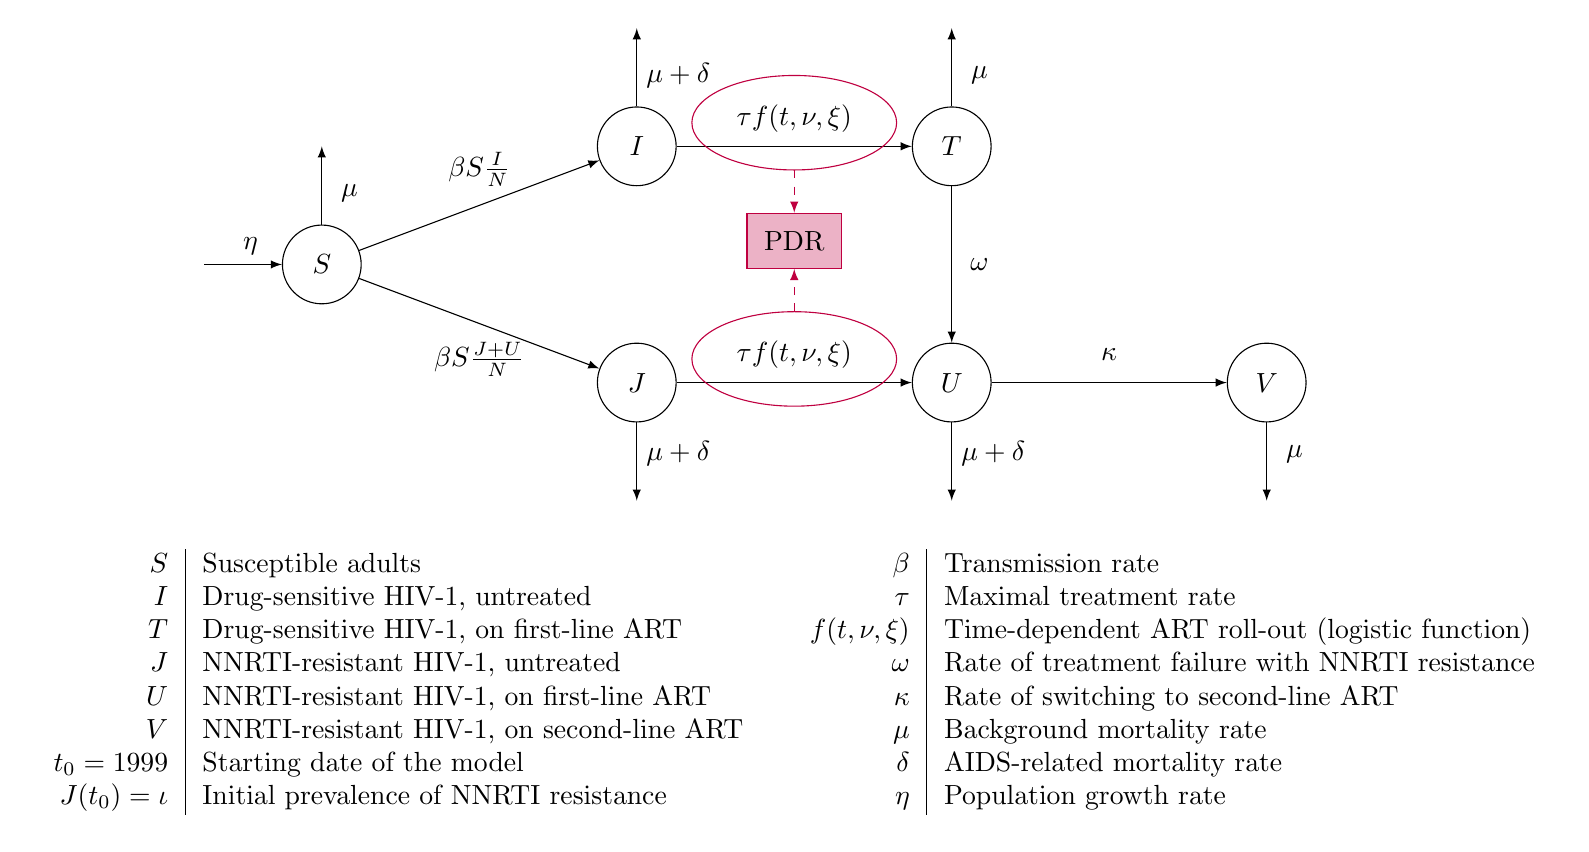
\begin{tikzpicture}
		% cascade of care
		\node[circle, draw, inner sep=0pt, minimum size=1cm] (S) at (0,.5) {$S$};
		\node[circle, draw, inner sep=0pt, minimum size=1cm] (I) at (4,2) {$I$};
		\node[circle, draw, inner sep=0pt, minimum size=1cm] (J) at (4,-1) {$J$};
		\node[circle, draw, inner sep=0pt, minimum size=1cm] (T) at (8,2) {$T$};
		\node[circle, draw, inner sep=0pt, minimum size=1cm] (U) at (8,-1) {$U$};
		\node[circle, draw, inner sep=0pt, minimum size=1cm] (V) at (12,-1) {$V$};
		
		\draw[->,>=latex] (S) edge node[yshift=13pt] { $\beta S \frac{I}{N}$} (I);
		\draw[->,>=latex] (S) edge node[yshift=-13pt] { $\beta S \frac{J+U}{N}$} (J);
		\draw[->,>=latex] (I) edge node[yshift=10pt] { $\tau f(t,\nu,\xi)$} (T);
		\draw[->,>=latex] (J) edge node[yshift=10pt] { $\tau f(t,\nu,\xi)$} (U);
		\draw[->,>=latex] (T) edge node[xshift=10pt] { $\omega$} (U);
		\draw[->,>=latex] (U) edge node[yshift=10pt] { $\kappa$} (V);
				% resistance among disease failure

		\draw[<-,>=latex] (S) -- ++(-1.5,0) node [above,pos=.4] {$\eta$};
		\draw[->,>=latex] (S) -- ++(0,1.5) node [xshift=10pt,pos=.4] {$\mu$};
		\draw[->,>=latex] (I) -- ++(0,1.5) node [xshift=15pt,pos=.4] {$\mu+\delta$};
		\draw[->,>=latex] (T) -- ++(0,1.5) node [xshift=10pt,pos=.4] {$\mu$};
		\draw[->,>=latex] (J) -- ++(0,-1.5) node [xshift=15pt,pos=.4] {$\mu+\delta$};
		\draw[->,>=latex] (U) -- ++(0,-1.5) node [xshift=15pt,pos=.4] {$\mu+\delta$};
		\draw[->,>=latex] (V) -- ++(0,-1.5) node [xshift=10pt,pos=.4] {$\mu$};

		\draw[color=purple] (6,2.3) ellipse (1.3cm and .6cm);
		\draw[color=purple] (6,-0.7) ellipse (1.3cm and .6cm);
		\node[rectangle, fill,color=purple!30,minimum size=.7cm,minimum width=1.2cm] (pp) at (6,0.8) { };
		\node[rectangle, draw,color=purple,minimum size=.7cm,minimum width=1.2cm] (pdr) at (6,0.8) {\textcolor{black}{PDR}};
		\draw[dashed,purple,->,>=latex] (6,1.7) -- (pdr);
		\draw[dashed,purple,->,>=latex] (6,-.1) -- (pdr);
		% legend
		\node (leg) at (6,-4.8) {
			\begin{tabular}{r|lp{0cm}r|l}
			$S$ & Susceptible adults & & $\beta$ & Transmission rate \\
			$I$ & Drug-sensitive HIV-1, untreated & & $\tau$ & Maximal treatment rate \\
			$T$ & Drug-sensitive HIV-1, on first-line ART & &	$f(t,\nu,\xi)$ & Time-dependent ART roll-out (logistic function)\\	
			$J$ & NNRTI-resistant HIV-1, untreated & & 	$\omega$ & Rate of treatment failure with NNRTI resistance \\
			$U$ & NNRTI-resistant HIV-1, on first-line ART & &	 $\kappa$ & Rate of switching to second-line ART  \\
			$V$ & NNRTI-resistant HIV-1, on second-line ART & & $\mu$ & Background mortality rate \\
			$t_0=1999$ & Starting date of the model &&$\delta$ & AIDS-related mortality rate \\
			$J(t_0)=\iota$ & Initial prevalence of NNRTI resistance&&	$\eta$ & Population growth rate \\ 
			\end{tabular}};
		\end{tikzpicture}}
	\end{center}

	We imposed a \alert{hierarchical structure} on the parameters related to NNRTI resistance ($\omega$ and $\iota$). The other parameters were independently estimated for each country. The model was considered in a Bayesian framework and implemented in \texttt{Stan} (Carpenter et al., 2017).

}

%----------------------------------------------------------------------------------------


%----------------------------------------------------------------------------------------
%	RESULTS 2
%----------------------------------------------------------------------------------------

\headerbox{Results}{name=results1,span=2,column=3,row=0}{ % To reduce this block to 1 column width, remove 'span=2'
	The model is able to describe the rise of NNRTI PDR in each country over 2000-2018, accounting for the local dynamics of HIV-1 transmission, of ART roll-out and of AIDS-related mortality:
	\vspace{-.5em}
	\begin{center}
		\hspace{-2em}\includegraphics[width=.95\textwidth]{../figures/poster_pdr_M6.pdf}
		\vspace{-1.1em}
		\captionof{figure}{Model fit (median posterior and 95\% credible interval) of NNTI PDR for southern Africa (2000-2018).}
	\end{center}
				\vspace{-.3em}
 Predicted levels of NNRTI PDR in 2018 ranged between 3.3\% (95\% credible interval 1.9 to 7.1\%) in Mozambique and 25.3\% (17.9 to 33.8\%) in Eswatini. \alert{The main driver of NNRTI PDR was the conjunction of high ART coverage with a high rate of treatment failure associated with NNRTI resistance}. The rate of treatment failure associated with NNRTI resistance ranged from 0.0009 per year (0 to 0.13) in Botswana to 0.22 per year (0.12 to 0.55) in the Republic of South Africa.
 
 	\vspace{-.5em}
 \begin{center}
 	\hspace{-2em}\includegraphics[width=.8\textwidth]{../figures/poster_f3.pdf}
 	\vspace{-1.1em}
 	\captionof{figure}{(A) Estimated timing and intensity of ART roll-out by country. (B) Median estimate of the rate of treatment failure associated with NNRTI resistance per year (TNFR, corresponding to parameter $\omega$).}
 \end{center}
 


}


\headerbox{Conclusion}{name=discussion,span=2,column=3,below=results1}{ % To reduce this block to 1 column width, remove 'span=2'
Even with the introduction of dolutegravir, NNRTIs will remain a central component of first-line regimen in southern Africa. Between-country comparison shows that \alert{NNRTI resistance can be controlled despite high levels of ART coverage, as has been shown in Botswana}, likely because of better patient management and lower exposure to ART before treatment initiation. Data on NNRT PDR and ART management is sparse in some countries of southern Africa, leading to uncertainty in the estimates.
}



\headerbox{}{name=foottext, column=0, span=5, above=bottom, headerborder=open,boxheaderheight=1pt, headershape=rectangle,boxshade=none}{
	
	\vspace{-.4em}
	\begin{tabular}{p{.4\linewidth}p{.4\linewidth}|p{.2\linewidth}}
		
		\tiny{Contact:\textbf{ Julien Riou}, julien.riou@ispm.unibe.ch;  www.iedea-sa.org \hspace{3\linewidth} 
			The The International Epidemiology Databases to Evaluate AIDS (IeDEA) is supported by the U.S. National Institutes of Health’s National Institute of Allergy and Infectious Diseases, the Eunice Kennedy Shriver National Institute of Child Health and Human Development, the National Cancer Institute, the National Institute of Mental Health, the National Institute on Drug Abuse, the National Heart, Lung, and Blood Institute, the National Institute on Alcohol Abuse and Alcoholism, the National Institute of Diabetes and Digestive and Kidney Diseases, the Fogarty International Center, and the National Library of Medicine: AsiaPacific, U01AI069907; CCASAnet, U01AI069923; Central Africa, U01AI096299; East Africa, U01AI069911; NA-ACCORD, U01AI069918; Southern Africa, U01AI069924; West Africa, U01AI069919. Informatics resources are supported by the Harmonist project, R24AI124872. This work is solely the responsibility of the authors and does not necessarily represent the official views of any of the institutions mentioned above.}
		& \tiny{ \textbf{IeDEA-Southern Africa Steering Committee}: Matthias Egger (co-PI), University of Bern, Switzerland; Mary-Ann Davies (co-PI), University of Cape Town, South Africa; Gary Maartens, Aid for AIDS, South Africa; Carolyn Bolton, Michael Vinikoor, Centre for Infectious Disease Research in Zambia (CIDRZ), Zambia; Robin Wood and Catherine Orrell, Gugulethu ART Programme, South Africa; Nosisa Sipambo, Harriet Shezi Clinic, South Africa; Frank Tanser, Africa Centre for Health \& Population Studies (Hlabisa), South Africa; Andrew Boulle, Khayelitsha ART Programme, South Africa; Geoffrey Fatti, Kheth’Impilo, South Africa; Sam Phiri, Lighthouse Clinic, Malawi; Cleophas Chimbetete, Newlands Clinic, Zimbabwe; Karl Technau, Rahima Moosa Mother and Child Hospital, South Africa; Brian Eley, Red Cross Children's Hospital, South Africa; Josephine Muhairwe, SolidarMed Lesotho; Juan Burgos-Soto, SolidarMed Mozambique; Cordelia Kunzekwenyika, SolidarMed Zimbabwe, Matthew P Fox, Themba Lethu Clinic, South Africa; Hans Prozesky, Tygerberg Academic Hospital, South Africa.}
		
		&
		\vspace{-.4em}
		
\includegraphics[height=1.6cm]{figures/ideasa.jpg} \hspace{.5em} 
\includegraphics[height=1.6cm]{figures/ublogo.pdf}\hspace{.5em}  
\includegraphics[height=1.6cm]{figures/logo_uct.png} \hspace{1em} \\
		
\end{tabular}
\vspace{-.4em}
}


\end{poster}

\end{document}